\documentclass[uplatex]{jsarticle}
\usepackage{amsmath}
\usepackage[dvipdfmx]{graphicx}

\setcounter{tocdepth}{3}
\usepackage{float}
\usepackage{moreverb}
\usepackage{lscape}
%\pagestyle{empty}
%\usepackage{wrapfig}
%\usepackage{url}
%\usepackage{EasyLayout}

\usepackage{ascmac}
%\usepackage{fancybx}

%\pagestyle{myheadings}

\begin{document}

\title{第8回レポート課題(再提出)}
\author{25G1051近藤巧望}
%\date{2025年5月22日}
\maketitle

\section{はじめに}

習志野市に10店舗を展開するCITスーパーは売上高の減少に悩まされている.

CITスーパーを統括するマネージャーは,売上高減少の原因について調査するために
顧客へのアンケート調査を実施した.

本調査の目的は,CITスーパーの売上高を向上させるため,顧客のニーズを把握し,改善点を明らかにすることである.

\section{手法}

\begin{table}[H]
\caption{アンケート調査の結果.
接客スコア,品揃えスコア,立地スコアの平均値と各店舗の売上高を示す.}
\label{table:1}
\centering
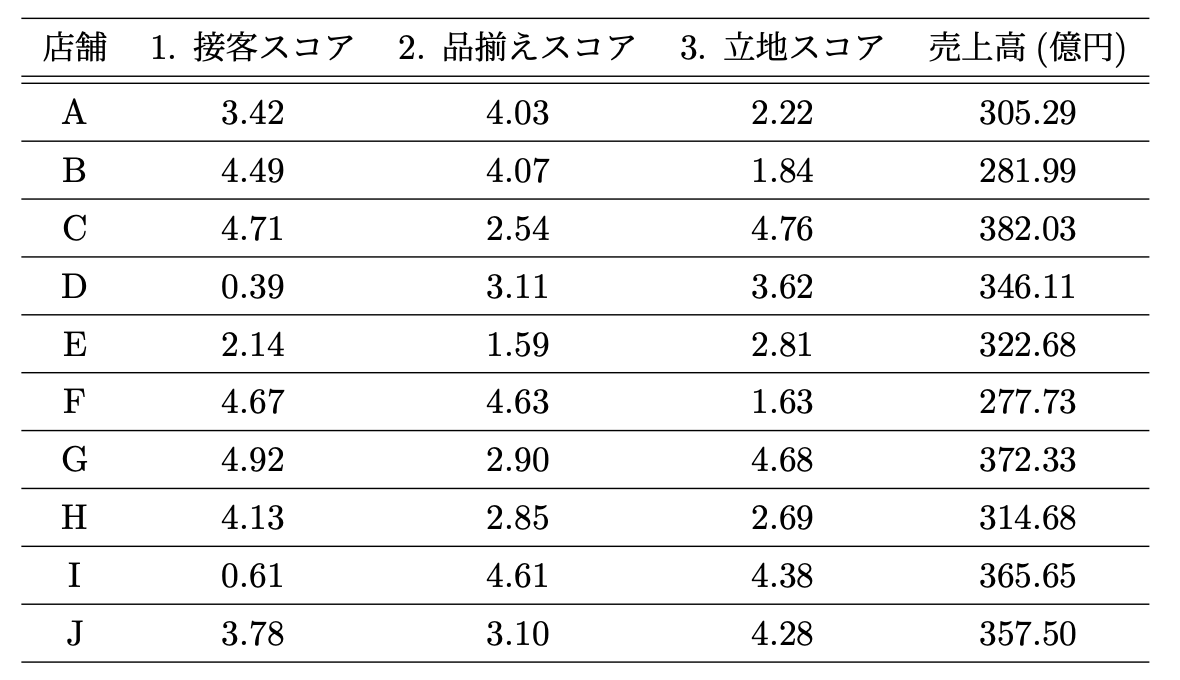
\includegraphics[width=8cm]{./Figs/table.png}
\end{table}

\indent
CITスーパーの顧客に,接客・品揃え・立地の項目から1から5の5段階評価でアンケート調査を行った.アンケート結果は表1のとおりである.
表1の結果から売上高減少の要因について分析し,最も効率よく売上高を改善する方法について考察する.

\section{結果}

\begin{figure}[H]
\centering
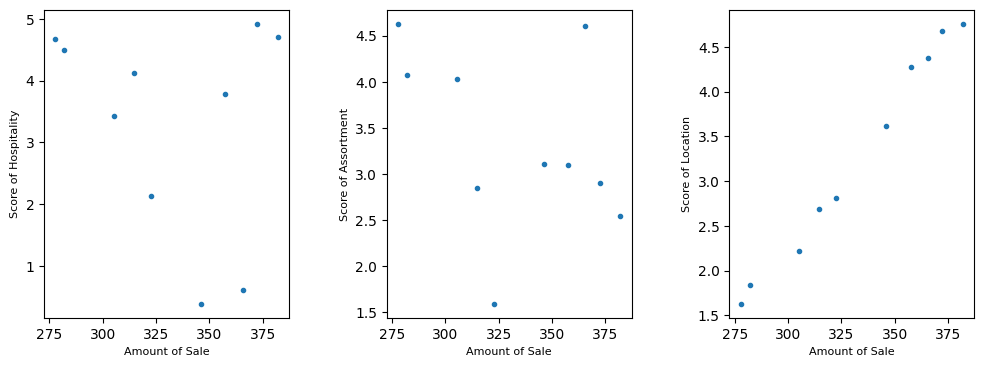
\includegraphics[width=8cm]{./Figs/scatter.png}
\caption{実施アンケートにおける各種スコアと売上高の散布図.
左から順に接客スコア,品揃えスコア,立地スコアと売上高の関係を表す.
これを見ると,立地スコアと売上高の間には正の相関があることがわかる.}
\label{fig:1-1}
\end{figure}

\indent
図1の散布図は,表1を元に接客スコア・品揃えスコア・立地スコアと売上高の間の関係を示したものである.
図1から,「接客スコアと売上高」「品揃えスコアと売上高」の散布図には,大きい相関は見られなかった.
一方で,「立地スコアと売上高」の散布図には大きい正の相関があることがわかった.

\section{おわりに}

\begin{table}[htb]
\centering
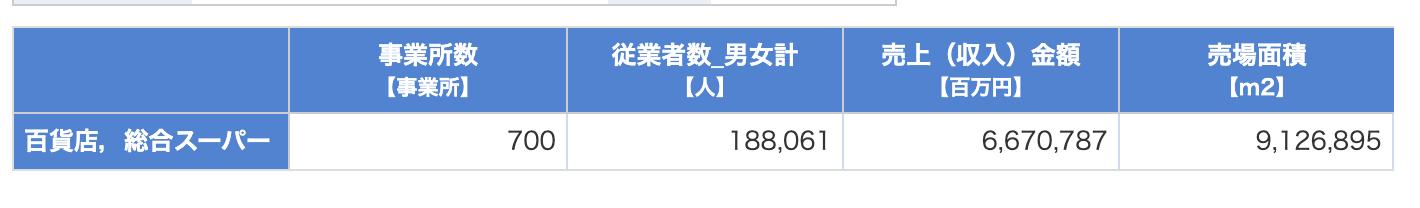
\includegraphics[width=8cm]{./Figs/syougyou.png}
\caption{全国の商業集積地区における百貨店・スーパーの事業所数,従業者数,売上金額,売上面積.(e-Stat Japan,https://www.e-stat.go.jp/dbview?sid=0004015860)
事業所数と売上金額ともに高水準であることが読み取れる.}
\label{table:2}
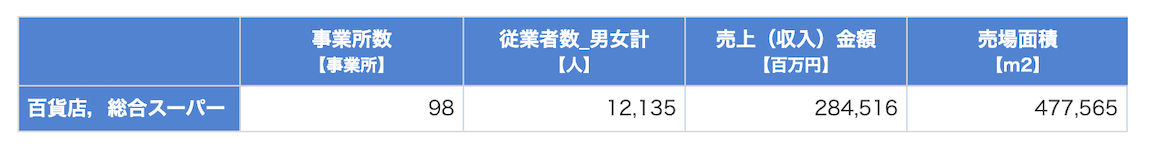
\includegraphics[width=8cm]{./Figs/kougyou.png}
\caption{全国の工業地区における百貨店・スーパーの事業所数,従業者数,売上金額,売上面積.(e-Stat Japan,https://www.e-stat.go.jp/dbview?sid=0004015860)
表2に比べると,事業所数と売上金額ともに低く,立地環境による影響を受けていることが考えられる.}
\label{table:3}
\end{table}

ここまででは,CITスーパーの売上高の減少の要因を明らかにするために顧客へのアンケート調査を行い,
その結果を図1に示し,立地と売上高に正の相関があることを突き止めた.

\indent
ここからは,立地と売上の関係について考察する.
まず図1の結果から,立地スコアが高くなるのに伴い売上高も高くなる傾向があることがわかる.
また,表2と表3が示す通り,商業集積地区においては百貨店・スーパーの事業所数と売上金額が高い水準にあるのに対し,
工業地区においては商業集積地区と比べ事業所数と売上金額が低い水準にある.
これらのことから,立地環境が売上高に影響を与えていることが考えられる.
したがって,CITスーパーの売上高を改善するためには,立地環境を改善することが最も効率的であると考えられる.

\indent
これらの結果と考察から,今後の課題として,立地環境を改善するための具体的な方法を検討する必要がある.
また,立地環境の改善に伴うコストと売上高の増加のバランスを考慮しながら,最適な改善策を見つけることが重要である.

\begin{thebibliography}{9}
\item e-Stat Japan, \textit{全国の商業集積地区における百貨店・スーパーの事業所数,従業者数,売上金額,売上面積}, https://www.e-stat.go.jp/dbview?sid=0004015860
\item e-Stat Japan, \textit{全国の工業地区における百貨店・スーパーの事業所数,従業者数,売上金額,売上面積}, https://www.e-stat.go.jp/dbview?sid=0004015860
\end{thebibliography}
\end{document}